% !TEX TS-program = pdflatex
% !TEX encoding = UTF-8 Unicode

% This is a simple template for a LaTeX document using the "article" class.
% See "book", "report", "letter" for other types of document.

\documentclass[11pt]{article} % use larger type; default would be 10pt

\usepackage[utf8]{inputenc} % set input encoding (not needed with XeLaTeX)

%%% Examples of Article customizations
% These packages are optional, depending whether you want the features they provide.
% See the LaTeX Companion or other references for full information.

%%% PAGE DIMENSIONS
\usepackage{geometry} % to change the page dimensions
\geometry{a4paper} % or letterpaper (US) or a5paper or....
% \geometry{margin=2in} % for example, change the margins to 2 inches all round
% \geometry{landscape} % set up the page for landscape
%   read geometry.pdf for detailed page layout information

\usepackage{graphicx} % support the \includegraphics command and options

% \usepackage[parfill]{parskip} % Activate to begin paragraphs with an empty line rather than an indent

%%% PACKAGES
\usepackage{booktabs} % for much better looking tables
\usepackage{array} % for better arrays (eg matrices) in maths
\usepackage{paralist} % very flexible & customisable lists (eg. enumerate/itemize, etc.)
\usepackage{verbatim} % adds environment for commenting out blocks of text & for better verbatim
\usepackage{subfig} % make it possible to include more than one captioned figure/table in a single float
% These packages are all incorporated in the memoir class to one degree or another...

%%% HEADERS & FOOTERS
\usepackage{fancyhdr} % This should be set AFTER setting up the page geometry
\pagestyle{fancy} % options: empty , plain , fancy
\renewcommand{\headrulewidth}{0pt} % customise the layout...
\lhead{}\chead{}\rhead{}
\lfoot{}\cfoot{\thepage}\rfoot{}

%%% SECTION TITLE APPEARANCE
\usepackage{sectsty}
\allsectionsfont{\sffamily\mdseries\upshape} % (See the fntguide.pdf for font help)
% (This matches ConTeXt defaults)

%%% ToC (table of contents) APPEARANCE
\usepackage[nottoc,notlof,notlot]{tocbibind} % Put the bibliography in the ToC
\usepackage[titles,subfigure]{tocloft} % Alter the style of the Table of Contents
\renewcommand{\cftsecfont}{\rmfamily\mdseries\upshape}
\renewcommand{\cftsecpagefont}{\rmfamily\mdseries\upshape} % No bold!

%%% END Article customizations

%%% The "real" document content comes below...

\title{Game Graphics Programming Project Document}
\author{Margaret Dorsey and Jesse Cooper}
%\date{} % Activate to display a given date or no date (if empty),
         % otherwise the current date is printed 

\begin{document}
\maketitle

\section{Project Documentation}

\subsection{Concept}
\par The main goal of the project is to showcase the various graphical and lighting
effects available within the engine, and to build an atmospheric environment for the player to explore. To this end, the actual functionality of the project is somewhat limited, and the design decisions of the project are mostly based on technical considerations, atmosphere building, cohesiveness, and exploration experience.
\par More specifically, the goal is the horror genre, and so the end goal of the effects we use and the environments we build is to contribute to a feeling of isolation, vulnerability, and terror.
\subsection{Inspiration and Reference}
\subsubsection{Related Titles}
The project is very similar to the Konami demo \textit{PT}, the indie title \textit{Gone Home}, and other similar titles, where the game is exploration based in a closed, highly scripted environment.
\subsubsection{Reference Material}
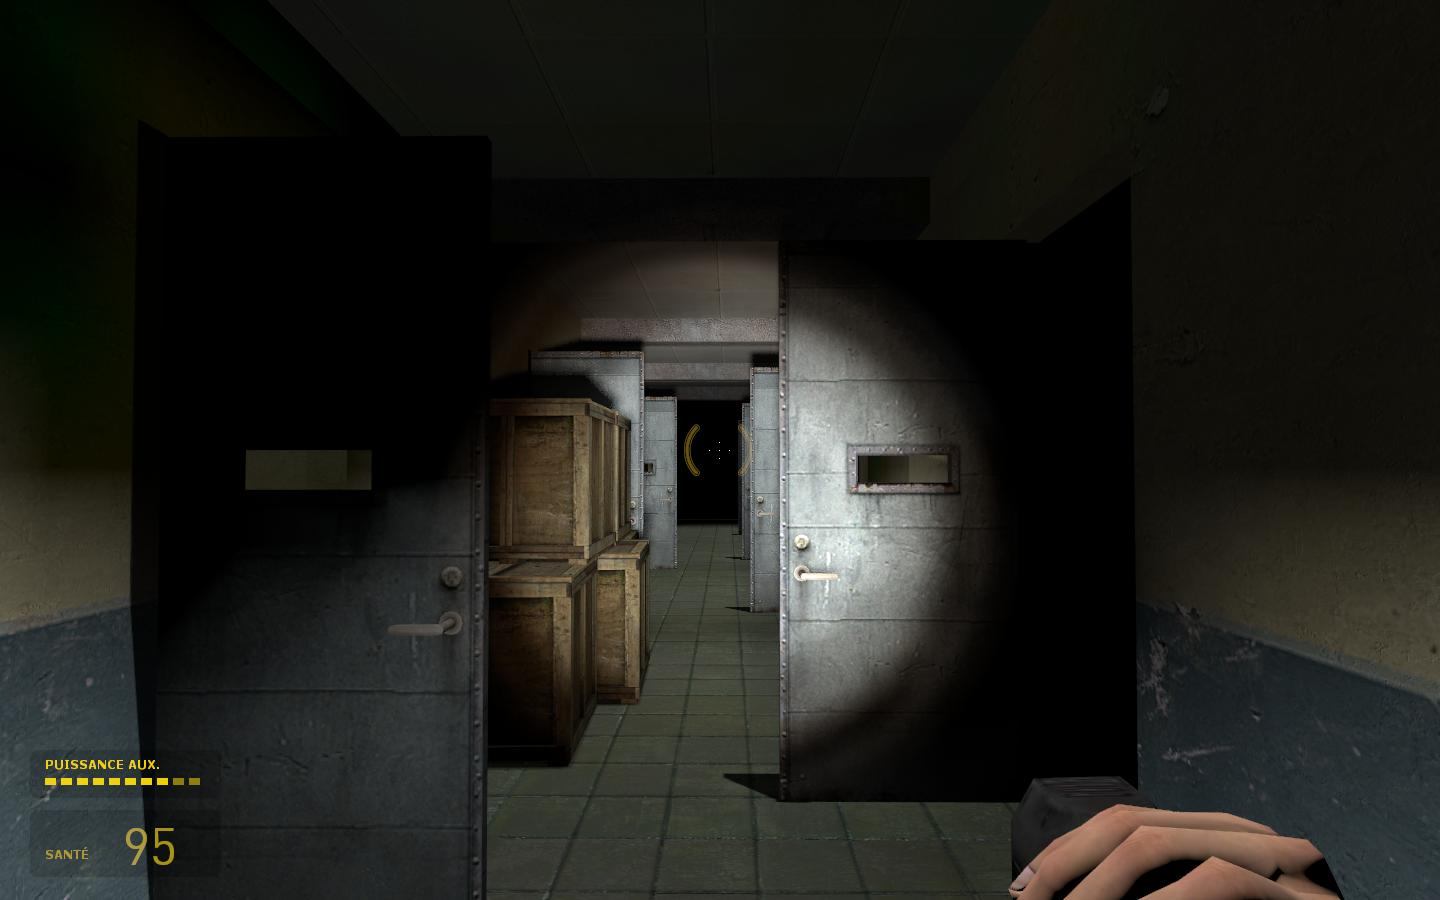
\includegraphics[scale=.2]{Media/flashlight.jpg} \\ \\
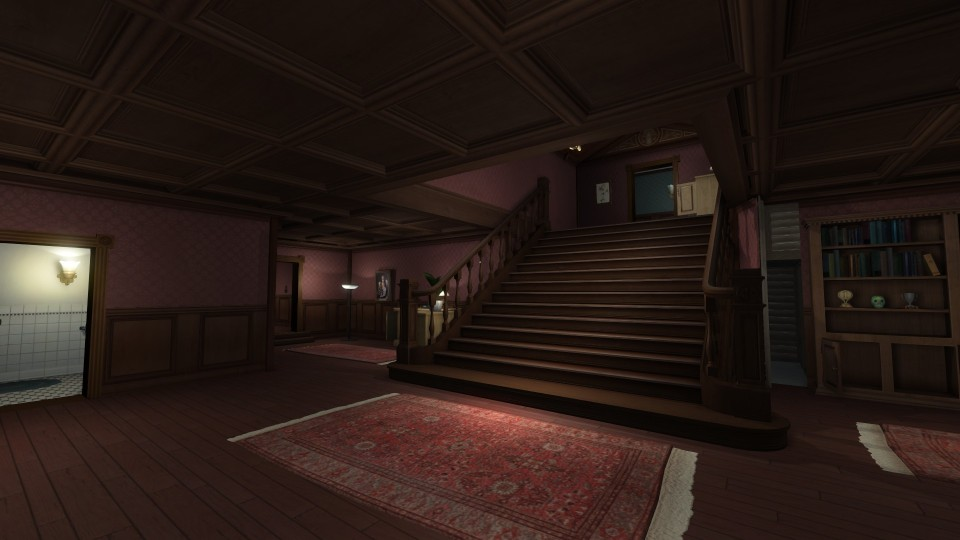
\includegraphics[scale=.3]{Media/gonehome1.jpg} \\ \\
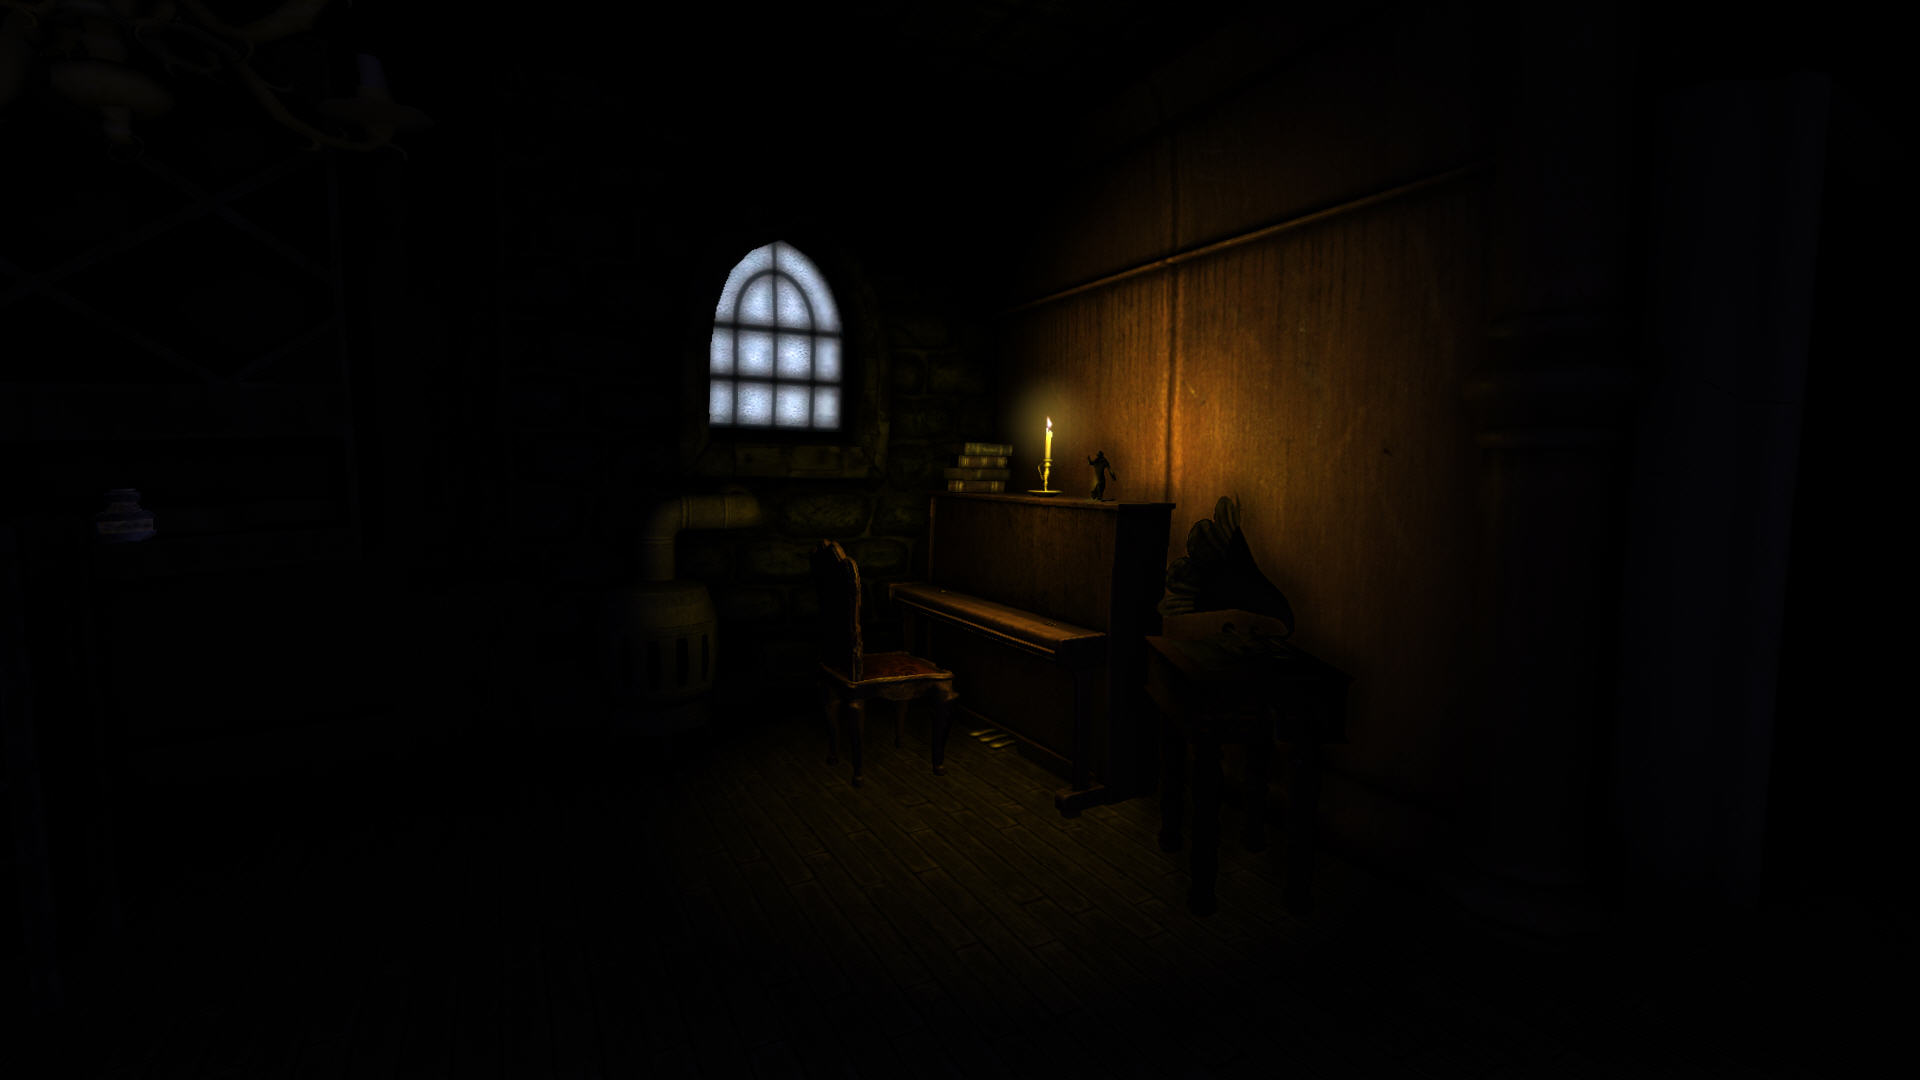
\includegraphics[scale=.2]{Media/insomniamod.jpg} \\ \\
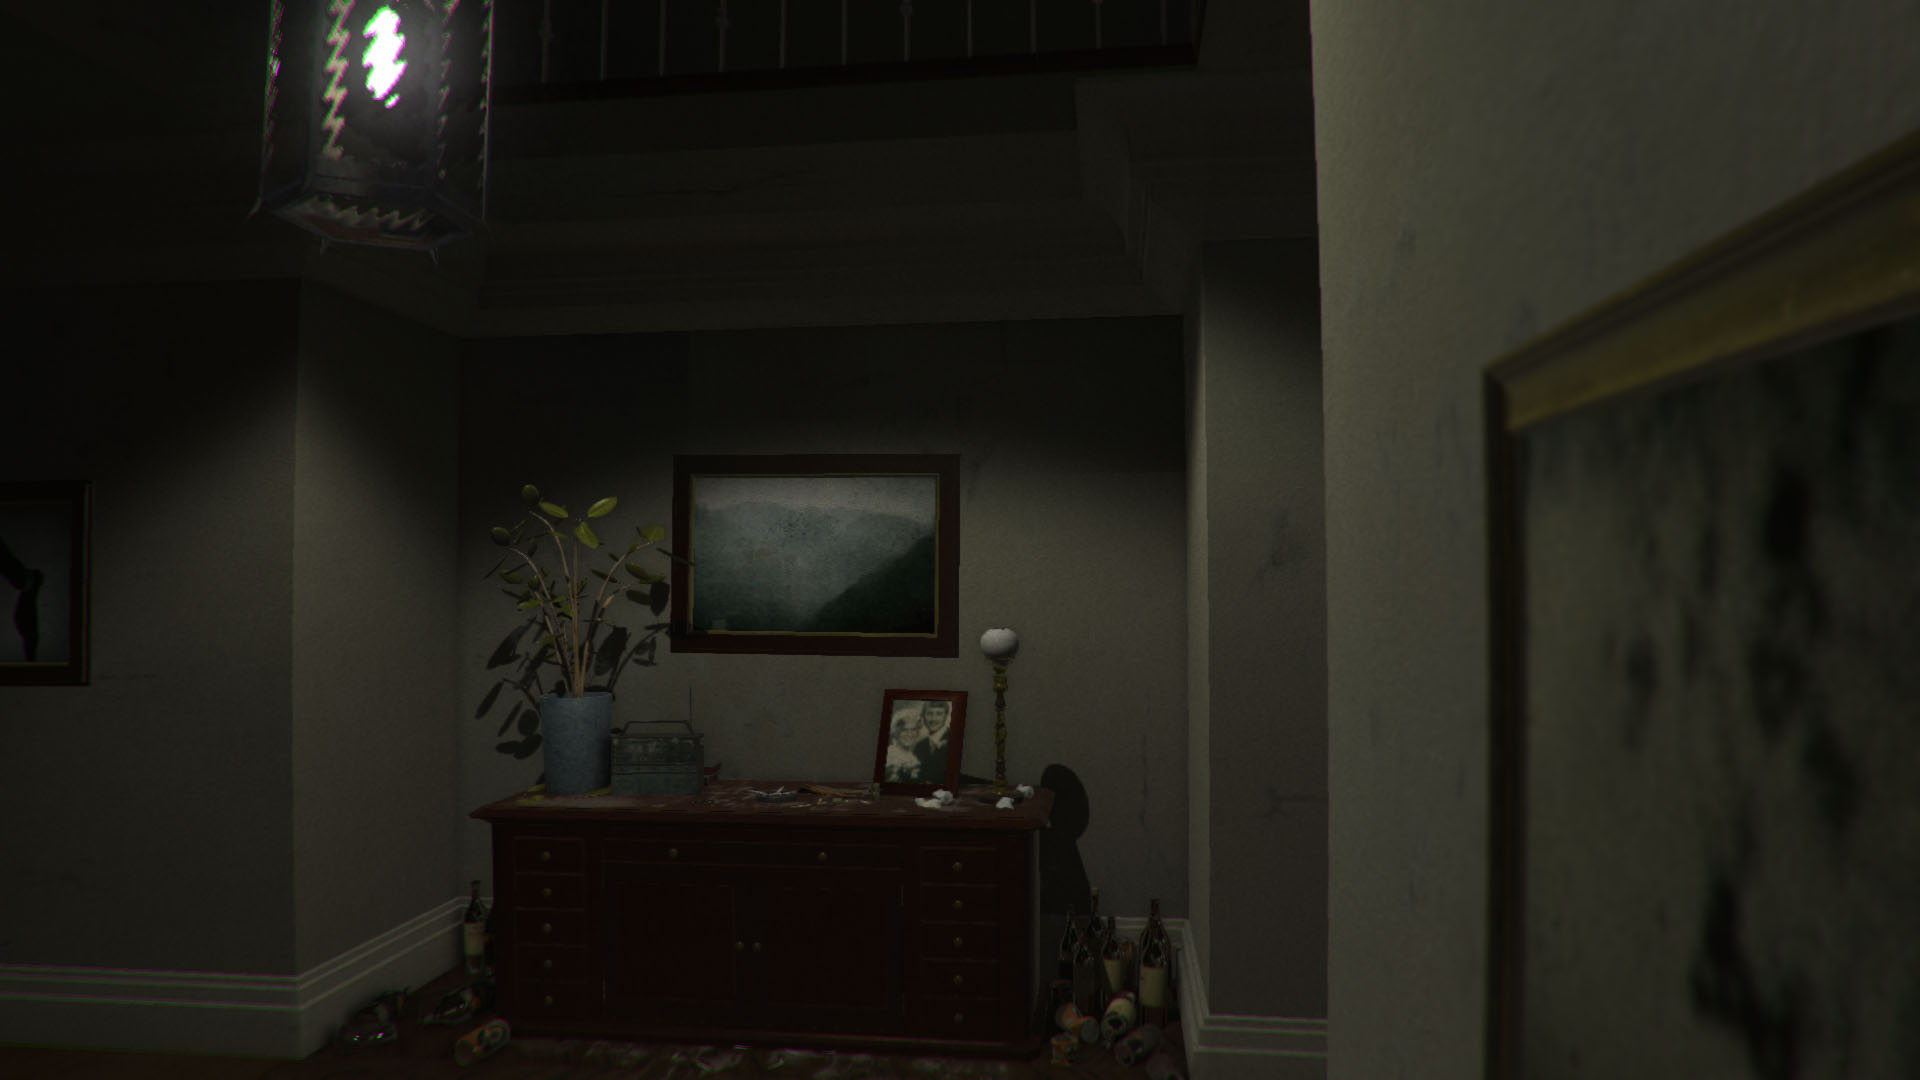
\includegraphics[scale=.2]{Media/pt2.jpg} \\
\subsection{Scope, Behavior and Technical Requirements}
The scope of the project is relatively small, given the relatively small time frame given by the class and our relative lack of development experience. The primary functionality will be simple collision detection and resolution, navigation of a 3d environment through a first person perspective, and dynamic changing of scenes and lighting (flashlight toggle) based on player behavior.

However, the technical requirements for rendering are significantly heavier - we will require at a minimum particle system generation and dynamic shadows. A list of tentative technical goals follows.

\begin{itemize}
\item Real Time Shadows
\item Fire, Smoke, Snow (Particle Systems)
\item Real Time Reflections (Glass, Metal, etc)
\item Water
\item Stretch Goals : Sound and Simple Animation
\end{itemize} 

\newpage
\section{Engine Documentation}

\subsection{Design and Target Functionality}
To suit the inherent modularity of the project, the engine is structured to dynamically
switch between pre-built scenes, provided in scene files, at runtime. This modularity allows
our engine to handle mid to high poly models and mid to high resolution textures, as well as a host of graphical effects, without the need for advanced optimization methods or a much deeper engine architecture. 
\par With this in mind, the scenes are constructed as parallel arrays of object information, in order to keep object data modular and expedite operations like collision checking, shader changes, or movement without costly cache misses. Additionally, scenes are loaded into a scene manager at runtime, where they can be dynamically switched between with virtually no load time - replacement is available without reindexing in case memory use becomes a concern.
\par Also thanks to the modularity of the architecture, it should be relatively simple to add new data to all objects for future graphics considerations without having to re-architect.
\subsection{Architecture Diagram}
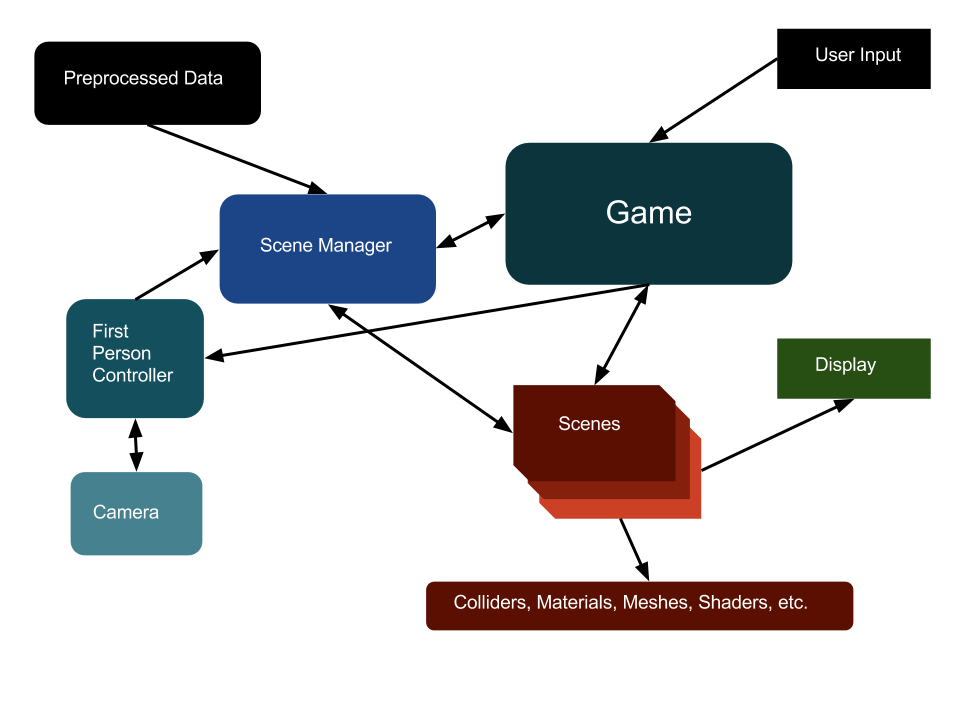
\includegraphics[scale=.4]{architecturediagram.png}
\subsection{Notes on Architecture}
Memory management is done through a reference system, so that Meshes, Materials, etc do not need to be duplicated to be reused, and \''ownership\'' of them need not be determined. The First Person Controller is `\''owned\'', built, and released by the Scene Manager. While in a more robust engine there would certainly be more dependencies, but luckily our structure can be kept relatively simple. 
\subsection{External Tools}
\par To reduce initial load times and the time cost of designing and implementing scenes, we will
 be building external tools that generate scene files, to be read by the scene manager to build the scene in engine, and rewrite the standard obj files to include binormal and tangent vectors, as well as a new set of indices to account for this extra data. As the project develops, this modified obj file may be expanded to include more data that can be precomputed outside of runtime.
\subsection{File Formats}

\subsubsection{Model File Format}
The model file format, .model, is a modified .obj format that includes binormal and tangent vectors per vertex. A sample .model file can be found in the Documentation directory of the project.
\subsubsection{Scene File Format}
The scene file format, .scene, contains all the meshes, textures, shaders, lights, and object and material information necessary to construct a scene. A sample .scene file can be found in the Documentation directory of the project.

\section{ Task List and Timetable}

\subsection{Task List}
\subsubsection*{End Goals}
\begin{itemize}
\item Working Collision
\item Working First Person Controller
\item Seamless Scene Swaps through Doors \& Staircases
\item External Tools
\item Particle Systems (Snow and Fire)
\item Real Time Shadows
\item House Layout/Design
\item Culling
\item Advanced Graphics Effects (to be added as they become feasible)
\end{itemize}
\subsubsection*{Implementation Dependency}
The external tools must be done before we can meaningfully build scenes, as writing scene files by hand is neither efficient nor intuitive. The house layout must also be at least roughed out before we can build the scenes. After the basic framework of the environment, as well as the FPC and the collision system are all implemented in engine, we actually have tremendous freedom to modularly add functionality as we desire, which will make division of work significantly simpler.
\renewcommand{\arraystretch}{1.4}
\subsection{Working Timetable}
\begin{tabular}{|l || l |}
\hline
\textbf{Week 3} & FPC, Collisions, Scene Loading Debugged\\
& Textures and Maps for Meshes \\
& External Tools \\
\hline
\textbf{Week 4} & House Design \& Build\\
		& Finish Base Game \\
		& Implement Real Time Shadows\\
		& Start on Particle System\\
\hline
\textbf{Week 5} & Seamless Scene Switching \\
 & Culling and Optimization \\
 \hline
\textbf{Following Weeks} & TBD\\
\hline
\end{tabular}

\subsection{Communication and Code Sharing}
Because we have a small team size, there is not much structure neccessary to facilitate communication and code sharing. The project source control through git doubles as 
code-sharing through github, and other files are shared through a Google Drive folder. Communication is primarily through text message and personal email.
\end{document}
